\subsection*{1 a)}

\textbf{Finn tiden $t_m$ når ballen faller ned på bakken ($y=0$) og
posisjonen $x(t_m) = x_m$ hvor dette skjer.}
\\
\\
Vi får oppgitt at:
\begin{align*}
    &x(t) = v_0t \cos{\theta}
    \\
    &y(t) = v_0t \sin{\theta} - \frac{1}{2}gt^2
\end{align*}

Vi vet at $t_m$ er når ballen treffer bakken. Det er når $y(t) = 0$.
Vi løser ligningen over for dette tilfellet:

\begin{align*}
    &y(t) = v_0t \sin{\theta} - \frac{1}{2}gt^2
    \\
    &0 = v_0t_m \sin{\theta} - \frac{1}{2}gt_m^2
    \\
    &v_0t_m \sin{\theta} = \frac{1}{2}gt_m^2
    \\
    &t_m = 2 \frac{v_0}{g}\sin{\theta}
\end{align*}

For å finne $x_m$ bruker vi $t_m$ i formelen for x(t):

\begin{align*}
    &x(t) = v_0t \cos{\theta}
    \\
    &x_m = v_0t_m \cos{\theta}
    \\
    &x_m = 2 \frac{v_0^2}{g}\sin{\theta} \cos{\theta}
\end{align*}


\subsection*{1 b)}

\textbf{Innfør dimensjonsløse variable $(x^*,y^*,t^*)$ for x,y,t når du skalerer
 med $x_m$ for lengde og $t_m$ for tid. Forklar hvorfor det ikke er behov for å
 skalere vinkelen $\theta$.}
\\
\\
Vi skalerer x og y med $x_m$ og t med $t_m$. Det gir:

\begin{align*}
    t^* = \frac{t}{t_m}
    \qquad
    x^* = \frac{x}{x_m}
    \qquad
    y^* = \frac{y}{x_m}
\end{align*}

% For $y_m$ velger jeg å skalere med toppunktet til $y(t)$.
% Det finner vi ved å sette inn en halv $t_m$ (fordi dette er en parabel
% og toppunktet halvveis mellom to ekvivalente verdier):
%
% \begin{align*}
%     &y(t) = v_0t \sin{\theta} - \frac{1}{2}gt^2
%     \\
%     &y(0.5t_m) = v_0\frac{v_0}{g}\sin{\theta} \sin{\theta}
%     - \frac{1}{2}g\frac{v_0^2}{g^2}\sin^2{\theta}
%     \\
%     &y(0.5t_m) = \frac{v_0^2}{g}\sin^2{\theta}
%     - \frac{1}{2}\frac{v_0^2}{g}\sin^2{\theta}
%     \\
%     &y(0.5t_m) = \frac{1}{2}\frac{v_0^2}{g}\sin^2{\theta}
% \end{align*}
%
% Dermed blir den dimensjonsløse variabelen for y:
%
% \begin{align*}
%     y^* = y/y(0.5t_m)
% \end{align*}


\pagebreak
\subsection*{1 c)}

\textbf{Bruk Matlab eller Python for å tegne abner ($x^*$,$y^*$) for tre
utkastvinkler $\theta_n$ for n = 1,2,3. Velg $0<\theta_1 < \frac{\pi}{4}$,
$\theta_2 = \frac{\pi}{4}$ og $\frac{\pi}{4} < \theta_3 < \frac{\pi}{2}$.
Tegn de tre banene i samme koordinatsystem, og angi hvilken bane som svarer
til hvilken utkastvinkel. Forklar hvorfor disse diagrammene kan brukes til
å finne ballens baner for forskjellige verdier av utgangsfart $v_0$ og
forskjellige verdier av g.}


\begin{figure}[H]
		\centering
		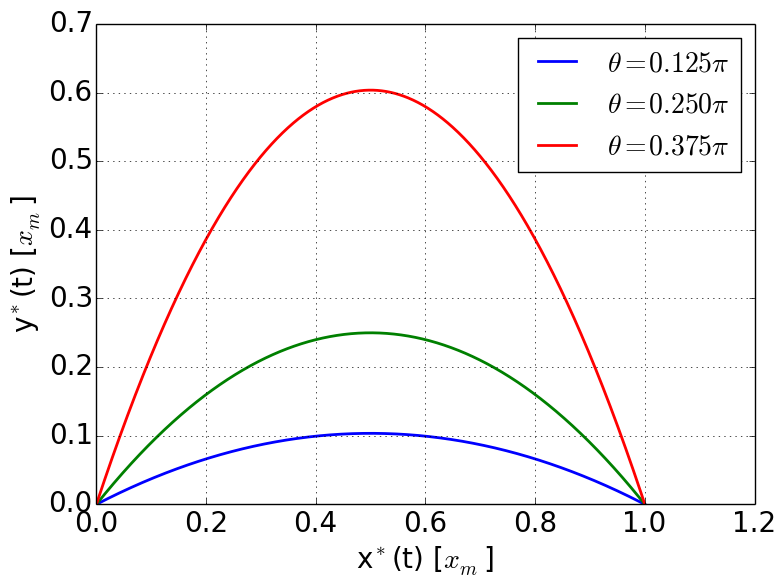
\includegraphics[width=0.7\linewidth]{../1a.png}
		\caption{Grafen viser hvordan banene til ballene med forskjellige
        utkastvinkel vil være i xy-planet. Programmet som ble brukt for
        å lage denne figuren finner du bakerst i innleveringen.}
		\label{fig_a1}
\end{figure}

Disse diagrammene kan brukes til å finne ballens baner for forskjellige verdier
av utgangsfart $v_0$ og forskjellige verdier av g. Trikset er at informasjonen
er lagret i aksene. Altså for at en skal kunne se på effekten av g og $v_0$, må en
pakke ut informasjonen fra aksene. De dimensjonsløse variablene gjør at
alle verdier for g og $v_0$ med samme utkastvinkel gir samme kurve.
